\documentclass[12pt]{article}
\usepackage{amsmath, amssymb, amsfonts, graphicx, geometry, float, caption, subcaption, booktabs}
\geometry{a4paper, margin=1in}

% Title and author setup without forced sizes
\title{PC3 Spectral Arbitrage: A PCA-Fourier Learning Model\vspace{1em}}

% Make the author section smaller using \small or \normalsize
\author{
    \small Danny Watkins \\ 
    \small MATH485: Mathematical Modeling \\ 
    \small The University of Arizona Department of Mathematics
}

\date{\small 2025}

\begin{document}

% Generate title
\maketitle

% Abstract with a slightly smaller font size for better readability
\begin{abstract}
\small
The U.S. Treasury yield curve encodes crucial information about economic conditions, with its shape driven by macroeconomic forces. Principal Component Analysis (PCA) reveals that yield curve shifts can be largely decomposed into three factors: level (PC1), slope (PC2), and curvature (PC3). This paper focuses on PC3, which captures localized deviations in mid-maturity bonds and exhibits mean-reverting behavior—making it a prime candidate for arbitrage. We employ PCA to extract PC3 dislocations, construct butterfly hedges to isolate them while neutralizing PC1 and PC2 exposure, and apply Fourier Transforms to smooth trading signals by filtering high-frequency noise. This paper rigorously derives the PCA decomposition, Fourier filtering methodology, and hedge ratio construction within a mathematical modeling framework, integrating empirical results from rolling PCA on 10 years of yield curve data to merge advanced mathematical techniques with practical financial applications.
\end{abstract}\vspace{1em}




\section{Introduction}

The U.S. Treasury yield curve is a foundational tool in finance, reflecting interest rates across maturities and signaling changes in economic conditions. While broad movements in the curve are primarily driven by macroeconomic forces, localized dislocations frequently emerge due to transient liquidity effects and supply-demand imbalances. These dislocations tend to revert to equilibrium, presenting opportunities for statistical arbitrage.To systematically capture and exploit these transient distortions, we employ \textbf{Principal Component Analysis (PCA)} to decompose the yield curve into its dominant movements. In essence, Principal Components (PCs) are mathematically derived patterns that emerge from the correlations among different bond maturities. Each PC represents an independent source of variation within the yield curve, ordered by the amount of variance they explain.\\

The first three components capture the majority of the yield curve's movement:
\begin{itemize}
    \item \textbf{PC1 (Level):} Represents parallel shifts in interest rates across all maturities, often driven by changes in monetary policy.
    \item \textbf{PC2 (Slope):} Reflects steepening or flattening of the curve, primarily affecting the short and long ends (the tails) of the curve.
    \item \textbf{PC3 (Curvature):} Captures deviations concentrated in the mid-maturities (the belly), relative to both short and long ends, driven by temporary market imbalances.
\end{itemize}

Among these components, PC3 (Curvature) exhibits mean-reverting behavior, making it particularly suitable for arbitrage strategies. Unlike PC1 (Level) and PC2 (Slope), which reflect broader economic shifts and systematic movements, PC3 dislocations represent more localized and transient mispricings. These residual variations typically manifest as localized distortions or transient bends in the yield curve, particularly in mid-maturity bonds. Unlike PC1 and PC2, which reflect more persistent economic trends, PC3 variations are often mean-reverting because they represent temporary dislocations that the market corrects over time.This inherent mean-reverting nature of PC3 makes it an attractive target for arbitrage. By isolating PC3 dislocations and constructing butterfly trades that neutralize PC1 and PC2 exposure, we aim to capture profit from the eventual reversion of these distortions to their equilibrium state.\\

To further refine trading signals, we apply \textbf{Fourier analysis} to filter high-frequency noise, enhancing the accuracy of trade execution. Additionally, we investigate machine learning methods such as \textbf{Long Short-Term Memory (LSTM) networks} and \textbf{Reinforcement Learning (RL)} to optimize trade timing and decision-making.\\

This project takes a mathematical modeling approach to yield curve arbitrage, rigorously deriving PCA decomposition, Fourier filtering techniques, and hedge ratio construction. By integrating advanced mathematical tools with empirical analysis of 10 years of historical yield curve data, we demonstrate the practical application of quantitative methods to arbitrage strategies in fixed-income markets.

\vspace{3em}

\section{Principal Component Analysis (PCA) in Yield Curve Analysis}

Principal Component Analysis (PCA) is a fundamental mathematical technique used to reduce the dimensionality of data while preserving its most significant patterns of variation. In the context of yield curve analysis, PCA decomposes the movements of interest rates across maturities into orthogonal components, each representing a distinct mode of variation. This decomposition reveals three principal components that dominate yield curve movements: Level (PC1), Slope (PC2), and Curvature (PC3).

The primary goal of this project is to isolate PC3, the curvature component, which captures localized distortions in mid-maturity bonds. These dislocations are inherently mean-reverting, making them suitable for arbitrage strategies. However, detecting and exploiting these signals in real time requires precise filtering to remove high-frequency noise and ensure consistent trade execution.



\subsection{Step-by-Step Breakdown of PCA (Concise Overview)}

To effectively utilize PCA in analyzing the yield curve, we break the process into the following concise steps:\\

\textbf{Step 1: Center the Data (Shift to the Origin)}
Before performing PCA, center the data by subtracting the mean from each observation. This ensures that the data has a mean of zero, stabilizing numerical computations.

\textbf{Step 2: Calculate the Covariance Matrix}
The covariance matrix quantifies pairwise relationships between features and captures how different maturities in the yield curve move relative to one another.

\textbf{Step 3: Extract Eigenvalues and Eigenvectors}
Compute the eigenvalues and eigenvectors of the covariance matrix to identify the principal components. Eigenvalues indicate the variance explained, while eigenvectors provide the direction of maximum variance.

\textbf{Step 4: Select Principal Components}
Choose the top principal components that capture the majority of the variance (typically PC1 and PC2). PC3 is specifically isolated for its mean-reverting qualities.

\textbf{Step 5: Project Data onto Selected Components}
Transform the original data by projecting it onto the selected principal components, reducing dimensionality while preserving significant patterns.



\subsection{Step-by-Step Mathematical Derivation of PCA}
\subsubsection{Step 1: Standardization of Data}
The first step in PCA is to standardize the data. This ensures that each feature has a mean of zero and a standard deviation of one. Standardization is essential because it eliminates the effects of differing scales between variables. The standardized data matrix \(X^*\) is calculated as:

\[
X^*_{ij} = \frac{X_{ij} - \mu_j}{\sigma_j}
\]

Where:
\begin{itemize}
    \item \(X_{ij}\) is the original value of feature \(j\) for sample \(i\).
    \item \(\mu_j\) is the mean of feature \(j\).
    \item \(\sigma_j\) is the standard deviation of feature \(j\).
\end{itemize}

\vspace{1em}

This step ensures that all variables have the same unit variance, allowing for comparison without the influence of differing scales.

\subsubsection{Step 2: Covariance Matrix Computation}
After standardizing the data, the next step is to compute the covariance matrix, which quantifies the pairwise relationships between standardized features:

\[
C = \frac{1}{n - 1} X^T X
\]

\vspace{1em}

The covariance matrix is symmetric, with diagonal elements representing variance and off-diagonal elements representing covariance between features. It captures how different maturities in the yield curve move in relation to each other.

\subsubsection{Step 3: Eigenvalue and Eigenvector Calculation}

Eigenvalues and eigenvectors are fundamental concepts in linear algebra that play a crucial role in Principal Component Analysis (PCA). An eigenvector of a square matrix is a nonzero vector that changes only in scale when that matrix is applied to it. In other words, the direction of the vector remains the same, but its magnitude may change. The scalar by which the eigenvector is scaled is called the eigenvalue.To decompose the covariance matrix, we compute its eigenvalues and eigenvectors. The eigenvalues represent the variance captured by each principal component, while the eigenvectors represent the directions of maximum variance. \\

The eigenvalue-eigenvector equation is given as:

\[
Av = \lambda v
\]

Rearranging the equation:

\[
(A - \lambda I)v = 0
\]

Where:
\begin{itemize}
    \item \(A\) is an \(n \times n\) matrix.
    \item \(I\) is the identity matrix of the same dimension.
    \item \(v\) is a nonzero vector.
    \item \(\lambda\) is the eigenvalue associated with \(v\).
\end{itemize}
\vspace{2em}

For a nontrivial solution (nonzero \(v\)), the determinant of \((A - \lambda I)\) must be zero:

\[
\text{det}(A - \lambda I) = 0
\]\\

This determinant equation is called the \textbf{characteristic equation}, and its roots are the eigenvalues of the matrix \(A\).\\

To find the eigenvalues and eigenvectors of the covariance matrix \(C\), we use the characteristic equation:

\[
\text{det}(C - \lambda I) = 0
\]


Where:
\begin{itemize}
    \item \(C\) is the covariance matrix.
    \item \(\lambda\) is the eigenvalue.
    \item \(I\) is the identity matrix.
\end{itemize}

\vspace{2em}

Solving this equation yields the eigenvalues that indicate the variance captured by each principal component. The corresponding eigenvectors provide the directions of maximum variance in the data. These components are crucial for projecting the original data onto a lower-dimensional space while retaining the most significant patterns of variation.


\subsubsection{Step 4: Select Principle Components}

After computing the eigenvalues and eigenvectors, the next step is to select the principal components that capture the most variance. The goal is to reduce dimensionality while preserving the most informative movements in the data. \\

To select the top principal components, we follow these steps:

\begin{enumerate}
    \item \textbf{Rank Eigenvalues:} Order the eigenvalues in descending order to determine which components capture the most variance.
    \item \textbf{Calculate Variance Explained:} Compute the proportion of variance explained by each eigenvalue:
    \[
    \text{Variance Explained} = \frac{\lambda_i}{\sum \lambda_j}
    \]
    Where:
    \begin{itemize}
        \item \(\lambda_i\) is the eigenvalue of the \(i\)-th principal component.
        \item \(\sum \lambda_j\) is the sum of all eigenvalues.
    \end{itemize}
    \item \textbf{Cumulative Variance:} Calculate the cumulative variance to determine how many components are needed to reach a desired threshold (e.g., 95\%):
    \[
    \text{Cumulative Variance} = \sum_{k=1}^{m} \frac{\lambda_k}{\sum \lambda_j}
    \]
    Where:
    \begin{itemize}
        \item \(m\) is the number of selected components.
    \end{itemize}
    \item \textbf{Retain Top Components:} Keep the principal components whose cumulative variance reaches the desired threshold (usually 95-99\%).
\end{enumerate}

Typically, the first few principal components capture the majority of the variance. In yield curve analysis, the first three components (PC1, PC2, PC3) often explain over 99\% of the variance, corresponding to the level, slope, and curvature movements, respectively.

\subsubsection{Step 5: Project Data and Principle Components}
Once the principal components are obtained through PCA, the next step is to project the original data onto these orthogonal axes. This transformation allows us to reduce dimensionality while retaining the most significant patterns of variation. The goal is to express the original data in terms of its principal components, where each component captures a portion of the variance. \\

The projection of the standardized data \(X^*\) onto the principal components is computed as:

\[
Z = X^* V
\]

Where:
\begin{itemize}
    \item \(X^*\) is the standardized data matrix.
    \item \(V\) is the matrix of eigenvectors (principal components).
    \item \(Z\) is the transformed data in the principal component space.
\end{itemize}

By projecting the data onto the principal components, we align the data along the orthogonal axes that capture the most variance, allowing for dimensionality reduction and enhanced interpretability.


\subsection{Example: PCA on Yield Curve Data}

To illustrate how PCA is applied to yield curve data, consider a simplified 2D example using two maturities (2-year and 10-year yields). The data matrix holds yield rates for each maturity at different time points. Each row corresponds to a specific date, and each column represents a maturity.

\subsubsection{Data Matrix}

\[
X = \begin{bmatrix} 
3.2 & 4.5 \\
3.5 & 4.6 \\
3.3 & 4.7 \\
3.1 & 4.8 \\
3.4 & 4.9 
\end{bmatrix}
\]

This data matrix represents five observations of two yield maturities (2Y and 10Y). To calculate the covariance matrix, we proceed as follows:

Calculating the mean of each column:

\[
\mu_1 = \frac{3.2 + 3.5 + 3.3 + 3.1 + 3.4}{5} = 3.3
\]

\[
\mu_2 = \frac{4.5 + 4.6 + 4.7 + 4.8 + 4.9}{5} = 4.7
\]

Centering the data by subtracting the mean from each value:

\[
X^* = X - \mu = \begin{bmatrix} 
3.2 - 3.3 & 4.5 - 4.7 \\
3.5 - 3.3 & 4.6 - 4.7 \\
3.3 - 3.3 & 4.7 - 4.7 \\
3.1 - 3.3 & 4.8 - 4.7 \\
3.4 - 3.3 & 4.9 - 4.7 
\end{bmatrix} = \begin{bmatrix} 
-0.1 & -0.2 \\
0.2 & -0.1 \\
0.0 & 0.0 \\
-0.2 & 0.1 \\
0.1 & 0.2 
\end{bmatrix}
\]

The covariance between two variables \(X\) and \(Y\) is calculated as:

\[
\text{Cov}(X, Y) = \frac{1}{n - 1} \sum_{i=1}^n (X_i - \mu_X)(Y_i - \mu_Y)
\]

Calculating the variance for the first variable:

\[
\text{Cov}(X, X) = \frac{1}{4} \left[(-0.1)^2 + (0.2)^2 + (0.0)^2 + (-0.2)^2 + (0.1)^2 \right] = 0.008
\]

Calculating the covariance between the two variables:

\[
\text{Cov}(X, Y) = \frac{1}{4} \left[(-0.1)(-0.2) + (0.2)(-0.1) + (0.0)(0.0) + (-0.2)(0.1) + (0.1)(0.2) \right] = 0.006
\]

Calculating the variance for the second variable:

\[
\text{Cov}(Y, Y) = \frac{1}{4} \left[(-0.2)^2 + (-0.1)^2 + (0.0)^2 + (0.1)^2 + (0.2)^2 \right] = 0.009
\]

Combining these values into the covariance matrix:

\[
C = \begin{bmatrix} 
0.008 & 0.006 \\
0.006 & 0.009 
\end{bmatrix}
\]

The covariance matrix quantifies how the two maturities move relative to each other. A positive covariance indicates that the yields tend to increase or decrease together, while a negative covariance would indicate opposite movements.



\subsubsection{Solving for Eigenvalues and Eigenvectors}

To find eigenvalues, we solve the characteristic equation:

\[
\text{det}(C - \lambda I) = 0
\]

For the covariance matrix:

\[
\text{det} \begin{bmatrix} 
0.008 - \lambda & 0.006 \\
0.006 & 0.009 - \lambda 
\end{bmatrix} = 0
\]

Expanding the determinant:

\[
(0.008 - \lambda)(0.009 - \lambda) - (0.006)^2 = 0
\]

\[
\lambda^2 - 0.017\lambda + 0.000036 = 0
\]

\subsubsection{Solving the Quadratic Equation}

Using the quadratic formula:

\[
\lambda = \frac{0.017 \pm \sqrt{0.017^2 - 4 \times 1 \times 0.000036}}{2 \times 1}
\]

\[
\lambda_1 = 0.014, \quad \lambda_2 = 0.003
\]

\subsubsection{Finding Eigenvectors}

For eigenvalue \(\lambda_1 = 0.014\), solving:

\[
(C - 0.014I)v = 0
\]

The solution yields:

\[
v_1 = \begin{bmatrix} 
0.707 \\
0.707 
\end{bmatrix}
\]

For eigenvalue \(\lambda_2 = 0.003\), solving:

\[
v_2 = \begin{bmatrix} 
-0.707 \\
0.707 
\end{bmatrix}
\]\\
\subsubsection{Example Results}

The eigenvalues obtained from PCA represent the amount of variance captured by each principal component, while the eigenvectors indicate the direction of maximum variance. In the context of yield curve analysis, understanding these components is crucial for interpreting the underlying movements of interest rates across maturities.

\paragraph{What Do the Eigenvalues Tell Us?}

The eigenvalues are directly associated with the variance explained by each principal component (PC). They quantify how much of the total variance in the yield curve data is captured by each component.

\paragraph{What Do the Eigenvectors Tell Us?}

The eigenvectors provide the directions in the original feature space (maturities) along which the variance is maximized. Each element within an eigenvector corresponds to a weight assigned to a particular maturity. Analyzing the eigenvector values helps us understand how different maturities contribute to each principal component.\\

For instance:
\begin{itemize}
    \item The eigenvector corresponding to PC1 generally has similar positive values across all maturities. This uniformity aligns with the idea of a parallel shift, where all yields move together in the same direction. It indicates that the level component affects all parts of the yield curve equally.
    \item The eigenvector corresponding to PC2 usually shows opposite signs for short-term and long-term maturities. This pattern reflects the tilting nature of the slope component, where short-term rates increase while long-term rates decrease (or vice versa).
    \item The eigenvector for PC3 often exhibits larger weights at mid-maturities compared to the tails (short and long ends). This demonstrates how PC3 captures localized dislocations in the belly of the curve, corresponding to a temporary steepening or flattening at intermediate maturities.
\end{itemize}

\paragraph{How Do Eigenvalues and Eigenvectors Combine?}

The combination of eigenvalues and eigenvectors tells us how \textbf{each principal component shapes the yield curve}:
\begin{enumerate}
    \item \textbf{PC1 Dominance}: The high variance captured by PC1 means that the most significant yield curve movements are level shifts. Any broad-based economic event (like a major policy change) that impacts the entire yield curve simultaneously will be predominantly explained by PC1.
    \item \textbf{PC2 Tilt}: The next most important movement involves steepening or flattening of the curve. Market reactions to expected changes in interest rate policies or inflation forecasts usually show up in PC2.
    \item \textbf{PC3 Distortion}: The smallest component, PC3, captures temporary and localized distortions, often driven by liquidity issues or short-term speculative activity. These deviations are typically mean-reverting, meaning they correct over time.
\end{enumerate}

\paragraph{Example Interpretation}

In our example, the calculated eigenvalues were:
\[
\lambda_1 = 0.014, \quad \lambda_2 = 0.003
\]

These eigenvalues indicate that \textbf{PC1 explains approximately 82\% of the variance} (\(0.014 / (0.014 + 0.003)\)), while \textbf{PC2 captures the remaining 18\%}. This strong dominance of PC1 aligns with the notion that level shifts are the primary drivers of yield curve movements.

The eigenvectors associated with these eigenvalues showed:
\begin{itemize}
    \item \textbf{PC1 Eigenvector:} \([0.707, 0.707]\) \\
    This indicates that both maturities (2Y and 10Y) move in the same direction and by similar magnitudes, reflecting a parallel shift.
    \item \textbf{PC2 Eigenvector:} \([-0.707, 0.707]\) \\
    This pattern shows that short and long maturities move in opposite directions, capturing a tilting effect.
\end{itemize}


\subsection{Conclusion}

The eigenvalues and eigenvectors derived from PCA provide a comprehensive understanding of yield curve dynamics. By analyzing both the \textbf{variance captured (eigenvalues)} and the \textbf{directions of movement (eigenvectors)}, we can effectively decompose the yield curve into its fundamental components: Level (PC1), Slope (PC2), and Curvature (PC3). The dominant yield curve shifts are primarily driven by level and slope changes, which reflect broad economic movements and changing market expectations.\\

Principal Component Analysis (PCA) offers a powerful mathematical approach to reducing the dimensionality of yield curve data while preserving its most significant movements. The first three principal components—level, slope, and curvature—effectively capture the dominant yield curve variations that reflect underlying economic forces. Focusing on PC3, which captures the curvature component, is essential because it represents localized, transient distortions in mid-maturity yields. Unlike PC1 and PC2, which reflect broader and more systematic shifts, PC3 dislocations represent temporary yield curve distortions that are inherently mean-reverting. These dislocations often arise from liquidity imbalances or short-term speculative activities, and they tend to self-correct as the market regains equilibrium. This understanding is fundamental for constructing butterfly trades that isolate PC3 by neutralizing PC1 and PC2 exposure which we will cover in a later section.

\vspace{3em}

\section{Implementing PCA on U.S. Treasury Yield Curve Data}

To effectively identify trading opportunities within the U.S. Treasury yield curve, we need to break down its movements into distinct components. Principal Component Analysis (PCA) enables us to isolate the curvature component (PC3), which captures localized, mean-reverting distortions. By separating PC3 from the dominant level (PC1) and slope (PC2) shifts, we can pinpoint transient dislocations that are ideal for arbitrage strategies. In this section, we detail how we performed PCA on real U.S. Treasury yield curve data, presenting both the methodology and the results. This foundational analysis sets the stage for generating trading signals explored later in the paper, including the use of Fourier analysis to smooth signals and the construction of butterfly hedge trades to isolate curvature-driven opportunities.

\subsection{Data Description}

The data used for our PCA analysis was obtained from the Federal Reserve Economic Data (FRED) API, covering a 10-year period from 2013 to 2023. It includes daily yields from the following maturities:
\begin{itemize}
    \item 3-month (3M), 6-month (6M), 1-year (1Y), 2-year (2Y)
    \item 5-year (5Y), 10-year (10Y), 20-year (20Y), 30-year (30Y)
\end{itemize}

These maturities represent a comprehensive range of short, intermediate, and long-term interest rates, allowing us to capture the full shape and evolution of the yield curve. The data was standardized to ensure that each maturity had a mean of zero and a standard deviation of one, preventing skewing by maturities with higher yield values.

\subsection{PCA Execution}

We performed PCA on the yield curve data to decompose the yield movements into orthogonal components. The primary objective was to isolate PC3 (curvature) while neutralizing the dominant PC1 (level) and PC2 (slope) effects. The key steps of the PCA execution are as follows:
\begin{enumerate}
    \item \textbf{Standardization:} Transforming the yield data to zero mean and unit variance to ensure comparability across maturities.
    \item \textbf{Covariance Matrix Calculation:} Computing the covariance matrix to quantify relationships between the standardized yield series.
    \item \textbf{Eigenvalue and Eigenvector Calculation:} Determining the variance captured by each principal component and the direction of maximum variance.
    \item \textbf{Projection onto Principal Components:} Transforming the standardized data into the principal component space.
    \item \textbf{Component Selection:} Retaining the top three principal components (PC1, PC2, PC3), which collectively explain over 99\% of the variance.
\end{enumerate}

\paragraph{Covariance Matrix}

Before applying PCA, we examine the covariance matrix to understand how each maturity moves relative to others. The covariance matrix quantifies the pairwise relationships between the yield series in their raw form. Unlike a correlation matrix, which standardizes values between -1 and 1, the covariance matrix reflects the actual covariances between maturities, capturing how movements in one yield relate to movements in another. \\

Our covariance matrix reveals distinct patterns based on maturity length:
\begin{itemize}
    \item \textbf{High Covariance in Short-Term Maturities:} The upper left section of the matrix (DGS3MO, DGS6MO, DGS1) exhibits bright yellow coloring, indicating high covariance. This means that short-term yields tend to move together strongly, often driven by monetary policy adjustments or short-term interest rate expectations.
    \item \textbf{Lower Covariance in Long-Term Maturities:} As maturities increase (toward DGS20 and DGS30), the covariance decreases, reflected in darker colors. Long-term yields are more independent, often influenced by different economic factors such as growth expectations and inflation.
    \item \textbf{Transitional Mid-Term Covariance:} Yields from DGS2 to DGS10 act as transitional points between short-term and long-term yields. This pattern shows how mid-term bonds blend characteristics of both short and long durations, responding to changes in both current interest rate environments and long-term economic outlooks.
\end{itemize}

\begin{figure}[H]
    \centering
    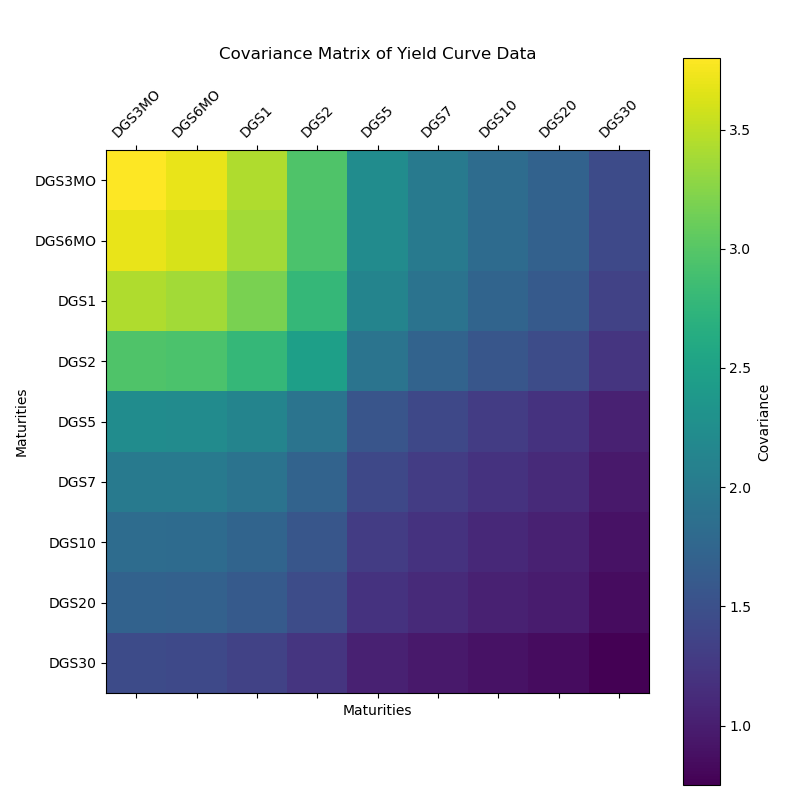
\includegraphics[width=0.8\textwidth]{visuals/covariance_matrix.png}
    \caption{Covariance Matrix of Yield Curve Data: Visualizing the pairwise covariances between different maturities. Covariance values reflect the degree to which yields move together, with larger values indicating stronger relationships. Short-term maturities exhibit higher covariance, while long-term maturities are less correlated, indicating more independent movements.}
    \label{fig:covariance_matrix}
\end{figure}



\subsection{Results and Visualizations}

Our PCA results demonstrated that the first three components capture the majority of the variance:
\begin{itemize}
    \item \textbf{PC1 (Level):} Captures approximately 90\% of the variance, representing parallel shifts across all maturities.
    \item \textbf{PC2 (Slope):} Accounts for around 8\% of the variance, indicating steepening or flattening of the curve.
    \item \textbf{PC3 (Curvature):} Explains about 1-2\% of the variance, capturing localized distortions in mid-maturity yields.
\end{itemize}

\begin{figure}[H]
    \centering
    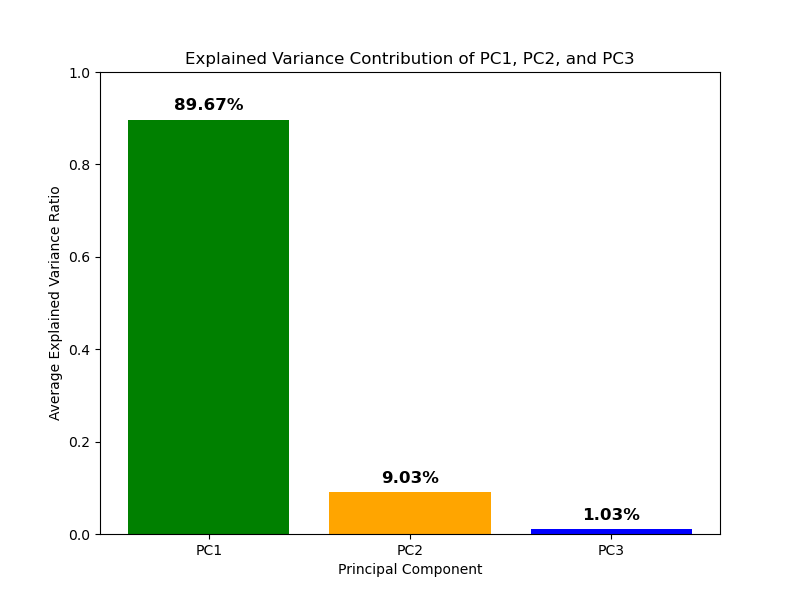
\includegraphics[width=0.8\textwidth]{visuals/pca_explained_variance.png}
    \caption{Explained Variance Contribution of Principal Components. PC1 accounts for 90.62\% of the variance, followed by PC2 with 8.19\% and PC3 with 0.93\%. These three components collectively capture the dominant yield curve movements, emphasizing the significance of level, slope, and curvature shifts.}
    \label{fig:pca_explained_variance}
\end{figure}


\paragraph{Geometric Interpretation}

To visually understand the transformation, we present the geometric interpretation of the data, showing both original vs. centered data in 2D and 3D.

\begin{figure}[H]
    \centering
    \begin{subfigure}[b]{0.48\textwidth}
        \centering
        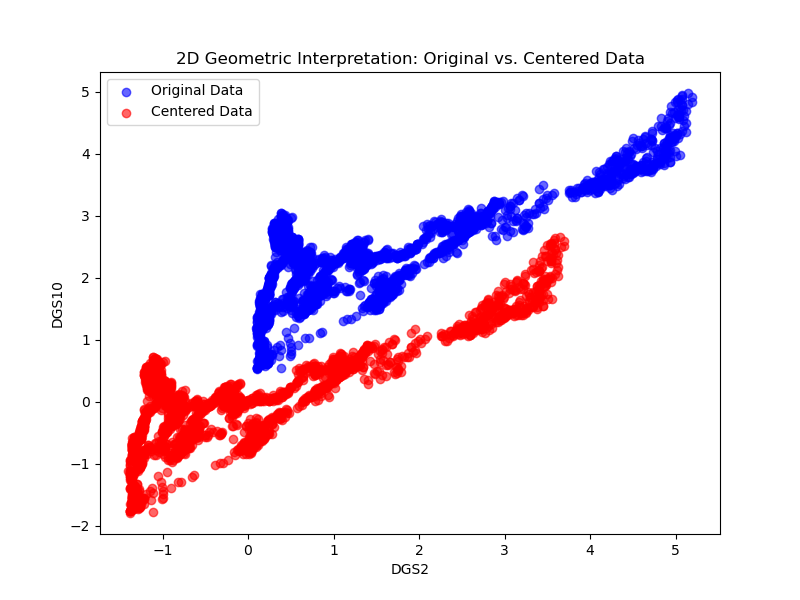
\includegraphics[width=\linewidth]{visuals/2d_geometric_interpretation.png}
        \caption{2D Geometric Interpretation: Original vs. Centered Data}
    \end{subfigure}
    \hfill
    \begin{subfigure}[b]{0.48\textwidth}
        \centering
        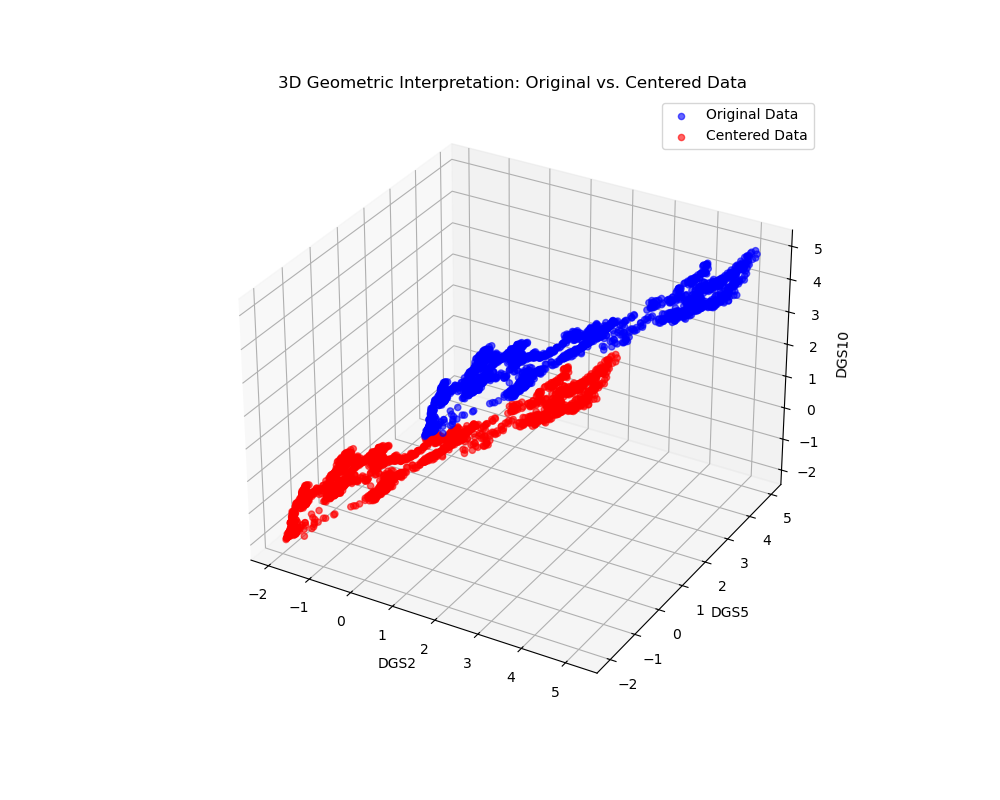
\includegraphics[width=\linewidth]{visuals/3d_geometric_interpretation.png}
        \caption{3D Geometric Interpretation: Original vs. Centered Data}
    \end{subfigure}
    \caption{Geometric Interpretation of Yield Curve Data: The left plot shows a 2D visualization comparing original and centered data, while the right plot extends the interpretation to three dimensions, highlighting the geometric transformation.}
    \label{fig:geo_int}
\end{figure}

\paragraph{Projection of Data onto Principal Components}

The projection visualizations illustrate how the data is transformed into the principal component space. The arrows in the 3D plot indicate the directions of the principal components (PC1, PC2, PC3).

\begin{figure}[H]
    \centering
    \begin{subfigure}[b]{0.48\textwidth}
        \centering
        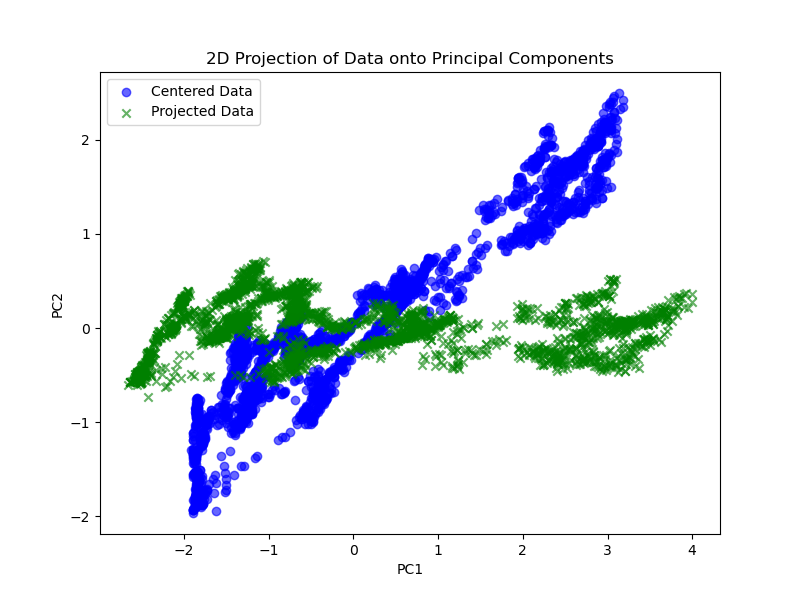
\includegraphics[width=\linewidth]{visuals/2d_projection_visualization.png}
        \caption{2D Projection onto Principal Components}
    \end{subfigure}
    \hfill
    \begin{subfigure}[b]{0.48\textwidth}
        \centering
        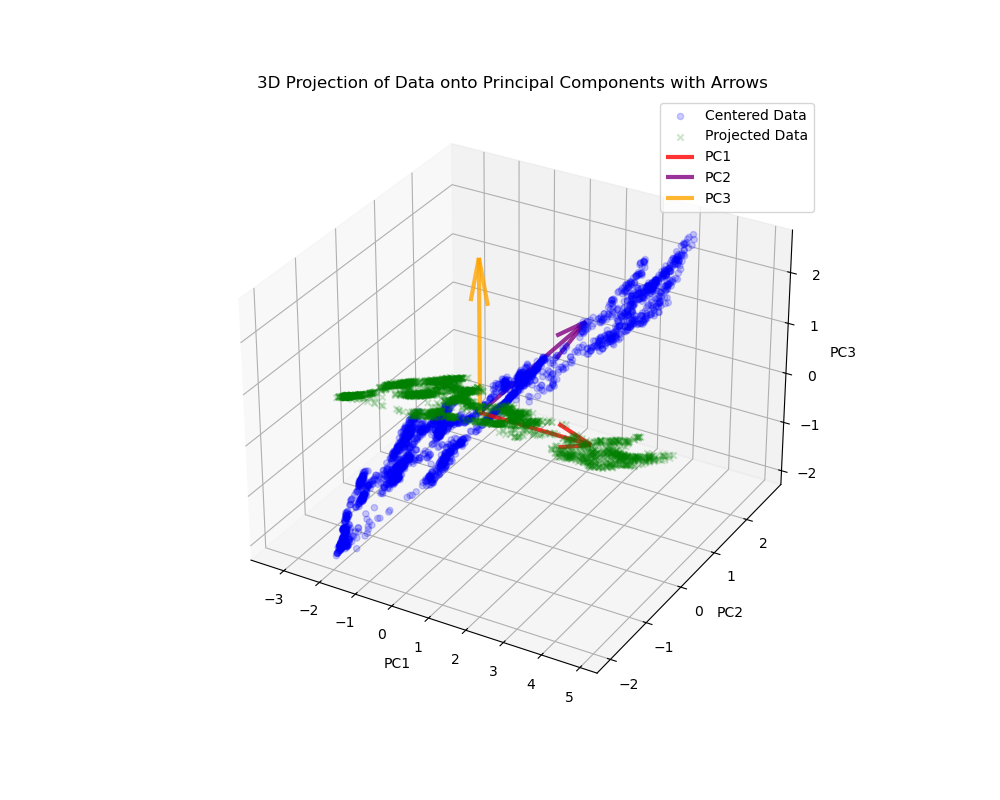
\includegraphics[width=\linewidth]{visuals/3d_projection_with_arrows.png}
        \caption{3D Projection with PC Arrows}
    \end{subfigure}
    \caption{Projection of Yield Curve Data onto Principal Components: The left plot shows a 2D projection of centered data, highlighting the transformation from raw space to PCA space. The right plot shows the 3D projection with arrows representing principal component directions.}
   \label{fig:projection_int}
\end{figure}

\subsection{Interpretation of Results}

The PCA analysis confirms that the yield curve dynamics are predominantly driven by:
\begin{itemize}
    \item \textbf{PC1 (Level)}: Uniform shifts across all maturities.
    \item \textbf{PC2 (Slope)}: Differential shifts between short and long maturities.
    \item \textbf{PC3 (Curvature)}: Transient distortions primarily affecting mid-maturities.
\end{itemize}

These results are consistent with the theoretical understanding that yield curve movements are mainly driven by level, slope, and curvature factors. The curvature component (PC3) is of particular interest as it captures localized, mean-reverting distortions, making it a prime candidate for arbitrage strategies. Isolating PC3 while neutralizing PC1 and PC2 will be the focus of subsequent stages of our project, including Fourier analysis and butterfly trade construction.

\section{Theoretical Justification of PC3 Mean-Reversion}

While PCA provides a mathematical decomposition of yield curve movements, understanding the economic and market microstructure factors driving PC3 dislocations is crucial for developing a robust arbitrage strategy. In this section, we explore the theoretical foundations of PC3’s mean-reverting behavior and verify its consistency across different market regimes. PC3, the curvature component, captures localized distortions in mid-maturity yields relative to short and long maturities. These dislocations often arise from temporary supply-demand imbalances or short-term market inefficiencies. Unlike parallel shifts (PC1) or slope changes (PC2), which may be driven by macroeconomic fundamentals, curvature dislocations are typically short-lived and driven by transient factors.

\subsection{Economic and Market Microstructure Factors}

Several factors contribute to the mean-reverting nature of PC3:

\begin{itemize}
    \item \textbf{Liquidity Imbalances:} Curvature dislocations often result from temporary liquidity constraints in intermediate maturities, where market participants are less active. This lack of participation can cause yields to deviate from their equilibrium, but as liquidity returns, the dislocation naturally corrects.
    \item \textbf{Flight-to-Safety Events:} During periods of market stress, investors may flock to long-term bonds, driving up long-end yields relative to mid-maturities. As market conditions stabilize, yield relationships typically revert to their mean, causing PC3 to correct.
    \item \textbf{Monetary Policy Effects:} Central banks often target short-term interest rates, leading to relatively stable short-end yields. Mid-maturity yields, however, are more susceptible to temporary dislocations due to policy uncertainty or forward guidance surprises.
    \item \textbf{Arbitrage Mechanisms:} Market makers and arbitrageurs exploit curvature dislocations by executing butterfly trades, which naturally force the yields back into alignment over time.
\end{itemize}

\subsection{Empirical Verification: Consistency Across Regimes}

To assess the mean-reverting behavior of PC3 dislocations, we analyzed their behavior across three distinct market regimes: low volatility, high volatility, and monetary policy changes. Our analysis focused on three key metrics: the half-life of PC3 dislocations, their correlation with the VIX (a measure of market volatility), and the statistical verification of mean reversion through the Augmented Dickey-Fuller (ADF) test.

\subsubsection{Half-Life of PC3 Dislocations}

The half-life measures the time it takes for a deviation from the mean to revert by half. A finite half-life indicates mean-reverting behavior, as deviations are temporary and eventually correct. Our results are as follows:

\begin{itemize}
    \item \textbf{Low Volatility:} 7.53 days
    \item \textbf{High Volatility:} 7.78 days
    \item \textbf{Monetary Policy Changes:} 1.98 days
\end{itemize}

These results demonstrate that PC3 dislocations revert to the mean in all regimes, with the fastest reversion occurring during monetary policy changes. This rapid correction suggests that PC3 dislocations are driven by transient market inefficiencies, which are quickly arbitraged away.

\subsubsection{Correlation with VIX}

We also examined the correlation between PC3 dislocations and the VIX to understand whether market volatility influences curvature distortions. The results are as follows:

\begin{itemize}
    \item \textbf{Low Volatility:} -0.19 (weak negative correlation)
    \item \textbf{High Volatility:} 0.15 (weak positive correlation)
    \item \textbf{Monetary Policy Changes:} 0.14 (weak positive correlation)
\end{itemize}

The weak correlations indicate that PC3 dislocations are largely independent of overall market volatility. Instead, they are driven by localized factors, such as liquidity imbalances or supply-demand dynamics in mid-maturity bonds. This independence further supports the idea that PC3 dislocations are mean-reverting, as they are not strongly influenced by broader market trends.

\subsubsection{Statistical Validation: Augmented Dickey-Fuller Test}

To statistically validate the mean-reverting nature of PC3 dislocations, we performed the Augmented Dickey-Fuller (ADF) test. This test assesses whether a time series is stationary, with the null hypothesis indicating the presence of a unit root (non-stationarity).

The ADF test results are as follows:

\begin{itemize}
    \item \textbf{ADF Statistic:} -5.29 (much lower than the critical value of -3.43 at 1\% significance)
    \item \textbf{p-value:} 5.85e-06 (extremely small, indicating strong evidence for mean reversion)
\end{itemize}

These results confirm that PC3 dislocations are statistically mean-reverting, providing additional validation for using PC3 as a basis for arbitrage strategies.

\subsection{Visualizations}

The visualizations in Figure~\ref{fig:multi_panel} demonstrate the findings of our analysis. The multi-panel visualization is designed to convey multiple aspects of PC3 mean reversion:

\begin{itemize}
    \item \textbf{Time Series Plot:} Shows the behavior of PC3 dislocations over time, highlighting different market regimes (low volatility, high volatility, and monetary policy changes).
    \item \textbf{Rolling Correlation Plot:} Visualizes the 30-day rolling correlation between PC3 dislocations and the VIX. The weak and fluctuating correlation throughout the period supports the conclusion that PC3 dislocations are independent of overall market volatility.
    \item \textbf{Correlation Heatmap:} Provides a comprehensive view of correlation coefficients between PC3 and VIX across different market regimes, highlighting the lack of strong associations.
    \item \textbf{Half-Life Bar Chart:} Quantifies the speed of mean reversion across regimes, emphasizing the rapid reversion during monetary policy changes.
\end{itemize}

\begin{figure}[H]
    \centering
    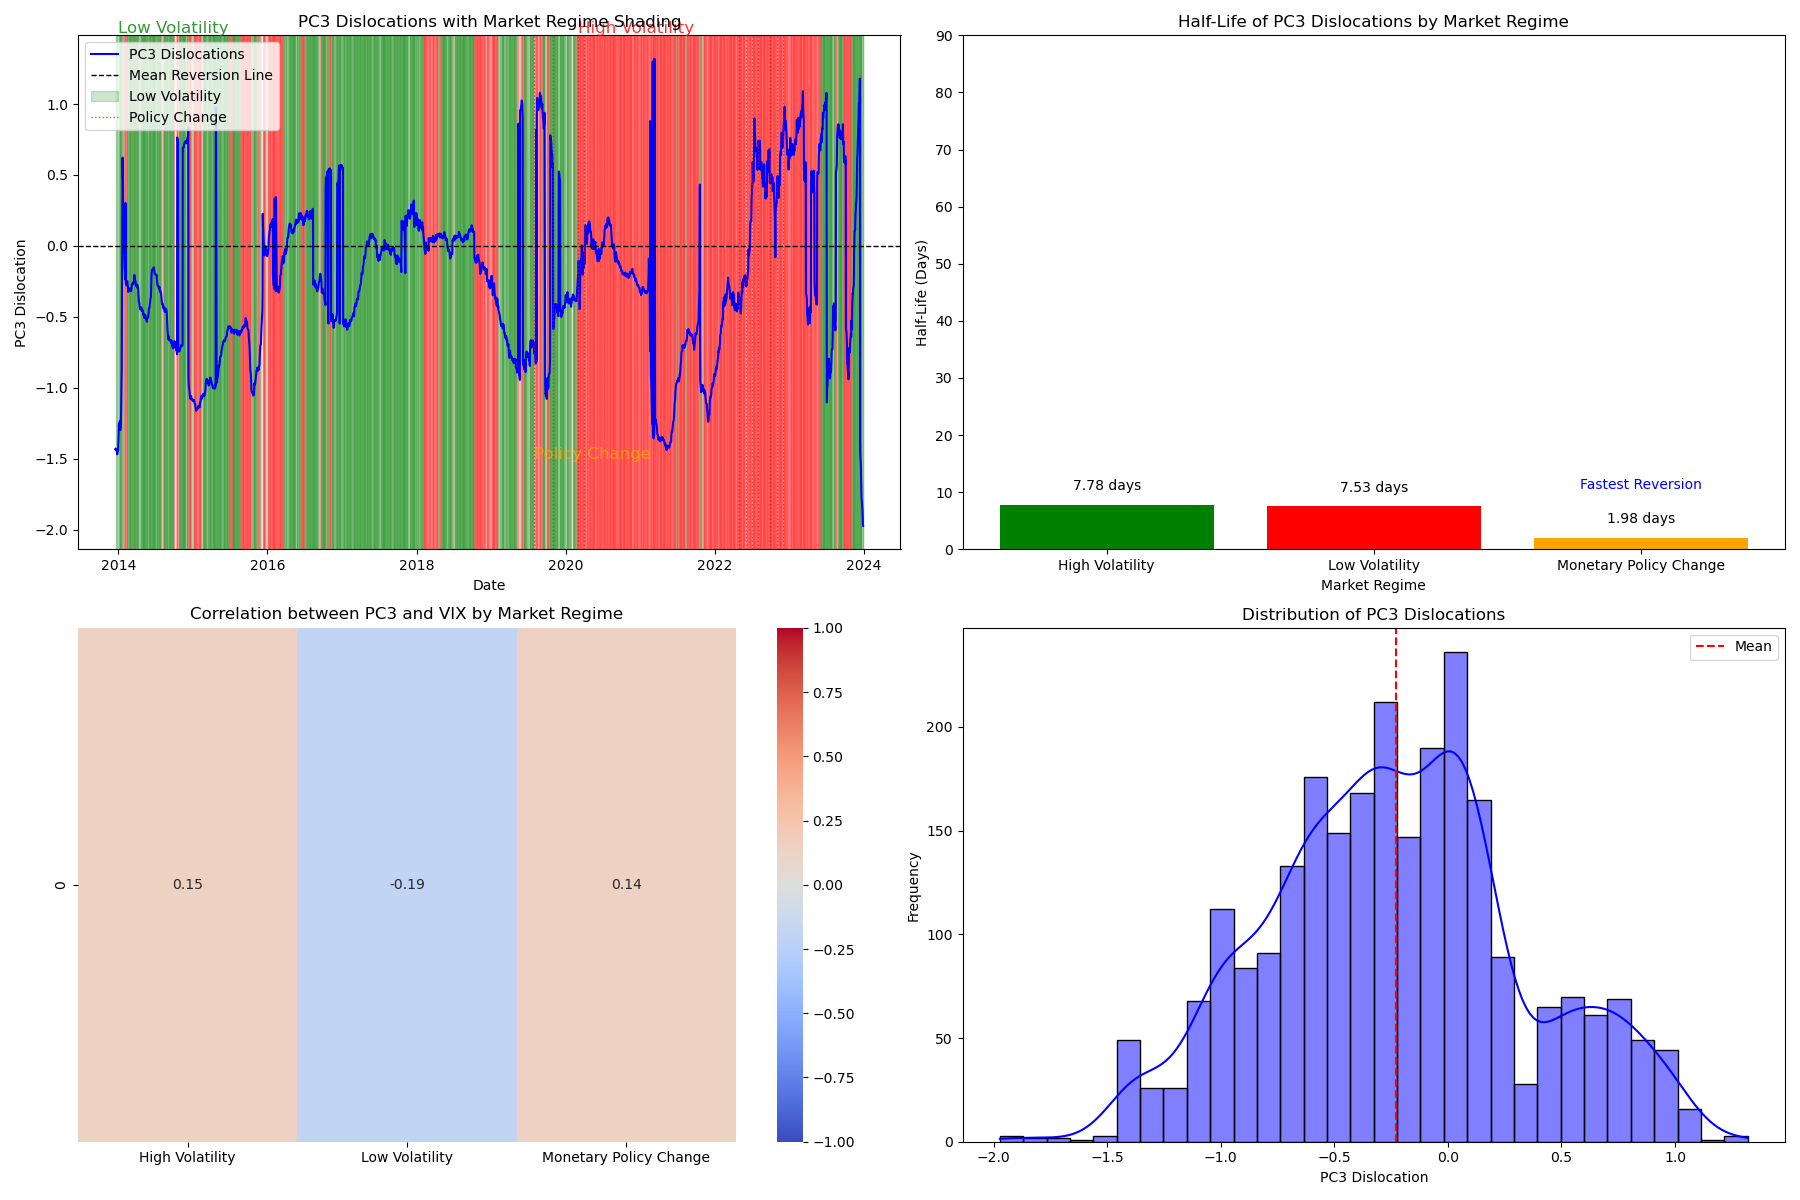
\includegraphics[width=\textwidth]{visuals/multi_panel_plot.png}
    \caption{Multi-panel visualization of PC3 dislocations across market regimes. The top-left panel shows the half-life of PC3 dislocations across low volatility, high volatility, and monetary policy change regimes. The top-right panel highlights the correlation between PC3 dislocations and the VIX. The bottom panels provide additional insights into the distribution of dislocations and policy change effects.}
    \label{fig:multi_panel}
\end{figure}

\subsection{Conclusion}

The foundational PCA analysis decomposes yield curve movements into orthogonal components that capture the dominant patterns of variation. By isolating PC3 and examining its characteristics, we gain a comprehensive understanding of localized, mean-reverting dislocations that present viable arbitrage opportunities. Our analysis confirms that PC3 dislocations exhibit strong mean-reverting behavior across all market regimes, with the fastest reversion occurring during periods of monetary policy change. This behavior highlights the transient nature of PC3-driven distortions, distinguishing them from broader market trends captured by PC1 and PC2. Additionally, the weak correlation between PC3 dislocations and the VIX suggests that curvature distortions are primarily driven by localized market dynamics rather than systemic volatility. These findings provide a strong theoretical foundation for the development of arbitrage strategies that specifically target PC3 dislocations. By isolating these transient opportunities while neutralizing systematic level and slope risks (PC1 and PC2), we can construct efficient butterfly trades that capitalize on mean reversion. The results obtained in this phase directly inform the next steps of our project, particularly the Fourier analysis and butterfly hedge construction, which will further refine trading signals and execution strategies.


\vspace{3em}



\section{Fourier Transform and Yield Curve Analysis}

\subsection{Introduction}
Fourier analysis is a mathematical technique that decomposes a signal into its constituent frequencies. It is particularly useful for identifying periodic or cyclical patterns in data, which can help in detecting seasonal effects, business cycles, or other recurring market dynamics. In the context of the yield curve, Fourier transforms help us understand the cyclical patterns in yield movements, allowing us to filter out noise and focus on the most significant trends.

Using Fourier transforms, we can analyze how the yield curve’s dislocations change over time and identify any cyclical behaviors that might exist. For instance, certain periods in the yield curve’s movement may be tied to seasonal economic effects, central bank policies, or other macroeconomic factors. By isolating these cyclical patterns, we can better understand when the yield curve is expected to revert to its "normal" state and uncover arbitrage opportunities.

\subsection{Mathematical Foundations}
The Fourier Transform allows us to represent a signal as a sum of sines and cosines with different frequencies. The fundamental concept behind Fourier analysis is to express a time-domain function as a superposition of sinusoidal functions, each with its own frequency, amplitude, and phase.

\subsubsection{Fourier Series Representation}
The Fourier series decomposes a periodic function $f(x)$ with period $T$ into a sum of sine and cosine terms:
\[
f(x) = A_0 + \sum_{n=1}^{\infty} \left[ A_n \cos \left( \frac{2\pi nx}{T} \right) + B_n \sin \left( \frac{2\pi nx}{T} \right) \right]
\]

Where:
- $A_0$ is the average (DC component),
- $A_n$ and $B_n$ are the Fourier coefficients,
- $T$ is the period of the function,
- $n$ is the harmonic number representing the frequency components.

\paragraph{Fourier Coefficients Calculation}
To calculate the Fourier coefficients, we use the following integrals:

\[
A_0 = \frac{1}{T} \int_{-T/2}^{T/2} f(x) \, dx
\]

\[
A_n = \frac{2}{T} \int_{-T/2}^{T/2} f(x) \cos \left( \frac{2\pi nx}{T} \right) \, dx
\]

\[
B_n = \frac{2}{T} \int_{-T/2}^{T/2} f(x) \sin \left( \frac{2\pi nx}{T} \right) \, dx
\]

These coefficients determine the strength of each frequency component in the dislocation signal. In our project, a high coefficient at a low frequency indicates a dominant long-term cycle in the yield curve curvature, suggesting persistent economic trends. High-frequency coefficients, on the other hand, typically represent noise or short-term fluctuations, such as transient market reactions or speculative activity. By filtering out these high-frequency components, we can focus on the most meaningful cyclical movements that reflect stable, mean-reverting dislocations.

\subsection{Discrete Fourier Transform (DFT)}
In practical applications, we work with discrete data rather than continuous functions. The Discrete Fourier Transform (DFT) is used to convert a sequence of time-domain data points into frequency components:

\[
X(k) = \sum_{n=0}^{N-1} x(n) \, e^{-\frac{2\pi ikn}{N}}
\]

Where:
- $X(k)$ is the frequency-domain representation,
- $x(n)$ is the time-domain data,
- $N$ is the number of data points,
- $k$ is the frequency index.

The frequency-domain representation tells us how much of each frequency is present in the original signal. Peaks in the magnitude of $X(k)$ correspond to dominant cycles or periodic patterns in the time-domain signal.



\paragraph{Interpretation and Practical Significance}
The reconstructed signal represents the smoothed PC3 dislocation time series. In practice, this means that the signal is cleaned of short-term noise, making it more reliable for trading applications. By isolating long-term cyclical patterns and minimizing noise, the filtered signal enhances the ability to predict reversion and to identify arbitrage opportunities more confidently.

\subsubsection{Example Calculation of DFT}
Let the time-domain signal be:
\[
x = [2, -1, 0, 1]
\]

To calculate the Discrete Fourier Transform (DFT), we use the formula:
\[
X(k) = \sum_{n=0}^{N-1} x(n) \, e^{-\frac{2\pi ikn}{N}}
\]

Here:
- \(x(n)\) represents the time-domain signal at index \(n\)
- \(N\) is the total number of data points (4 in this case)
- \(k\) is the frequency index (ranging from 0 to 3)

We calculate each frequency component as follows:

\paragraph{Step 1: Calculate \(X(0)\)}
Substituting \(k = 0\) in the DFT formula:
\[
X(0) = \sum_{n=0}^{3} x(n) \, e^{-\frac{2\pi i \cdot 0 \cdot n}{4}}
\]
Since the exponent becomes zero, the equation simplifies to:
\[
X(0) = 2 + (-1) + 0 + 1 = 2
\]
This shows that \(X(0)\) is simply the sum of all time-domain values.

\paragraph{Step 2: Calculate \(X(1)\)}
Substituting \(k = 1\) in the DFT formula:
\[
X(1) = \sum_{n=0}^{3} x(n) \, e^{-\frac{2\pi i \cdot 1 \cdot n}{4}}
\]
Expanding the sum:
\[
X(1) = 2 \, e^{0} + (-1) \, e^{-\frac{2\pi i}{4}} + 0 \, e^{-\frac{4\pi i}{4}} + 1 \, e^{-\frac{6\pi i}{4}}
\]
Using Euler's formula \(e^{-i\theta} = \cos(\theta) - i \sin(\theta)\), we have:
\[
e^{-\frac{2\pi i}{4}} = \cos\left(\frac{\pi}{2}\right) - i \sin\left(\frac{\pi}{2}\right) = 0 - i = -i
\]
\[
e^{-\frac{6\pi i}{4}} = \cos\left(\frac{3\pi}{2}\right) - i \sin\left(\frac{3\pi}{2}\right) = 0 + i = i
\]
Substituting these values:
\[
X(1) = 2 - (-i) + 0 + i = 2 + 2i
\]

\paragraph{Step 3: Calculate \(X(2)\)}
Substituting \(k = 2\) in the DFT formula:
\[
X(2) = \sum_{n=0}^{3} x(n) \, e^{-\frac{2\pi i \cdot 2 \cdot n}{4}}
\]
Expanding the sum:
\[
X(2) = 2 \, e^{0} + (-1) \, e^{-\frac{4\pi i}{4}} + 0 \, e^{-\frac{8\pi i}{4}} + 1 \, e^{-\frac{12\pi i}{4}}
\]
\[
e^{-\frac{4\pi i}{4}} = \cos(\pi) - i \sin(\pi) = -1
\]
\[
e^{-\frac{12\pi i}{4}} = \cos(3\pi) - i \sin(3\pi) = -1
\]
Therefore:
\[
X(2) = 2 + 1 + 0 - 1 = 2
\]

\paragraph{Step 4: Calculate \(X(3)\)}
Substituting \(k = 3\) in the DFT formula:
\[
X(3) = \sum_{n=0}^{3} x(n) \, e^{-\frac{2\pi i \cdot 3 \cdot n}{4}}
\]
Expanding the sum:
\[
X(3) = 2 \, e^{0} + (-1) \, e^{-\frac{6\pi i}{4}} + 0 \, e^{-\frac{12\pi i}{4}} + 1 \, e^{-\frac{18\pi i}{4}}
\]
\[
e^{-\frac{6\pi i}{4}} = \cos\left(\frac{3\pi}{2}\right) - i \sin\left(\frac{3\pi}{2}\right) = 0 + i = i
\]
\[
e^{-\frac{18\pi i}{4}} = \cos\left(\frac{9\pi}{2}\right) - i \sin\left(\frac{9\pi}{2}\right) = 0 + i = i
\]
Thus:
\[
X(3) = 2 - i + 0 + i = 2
\]

The resulting frequency-domain representation is:
\[
X = [2, 2 + 2i, 2, 2]
\]

This calculation shows how each frequency component of the original time-domain signal is transformed into a corresponding complex number in the frequency domain. Each value represents the amplitude and phase of a specific frequency component present in the original signal. Low-frequency components correspond to long-term trends, while high-frequency components capture short-term variations or noise. By decomposing the signal in this way, we gain insights into the dominant periodic patterns embedded within the data.




\section{Fourier Transform Implementation}

\subsection{Objective}
The primary goal of applying Fourier analysis in this project is to refine the output of our Principal Component Analysis (PCA) by filtering high-frequency noise from the PC3 dislocation signal. PCA identifies the curvature component (PC3) of the yield curve, which captures localized distortions in mid-maturity yields. However, PC3 dislocations often contain both meaningful long-term cyclical patterns and transient high-frequency noise. By applying Fourier Transform, we decompose the PC3 time series into its frequency components, enabling us to isolate and retain the low-frequency trends that signify significant cyclical behavior while filtering out noise. This step is essential to enhance the signal's robustness and clarity, ultimately improving the quality of arbitrage signals generated from PC3 dislocations.

\subsection{Data Processing}
The data input for the Fourier Transform consists of the PC3 dislocation time series, derived from our PCA on the yield curve data. The series reflects the curvature changes that occur independently of level and slope movements. The original PC3 dislocation series is shown in Figure~\ref{fig:pc3dislocation}.

\begin{figure}[H]
    \centering
    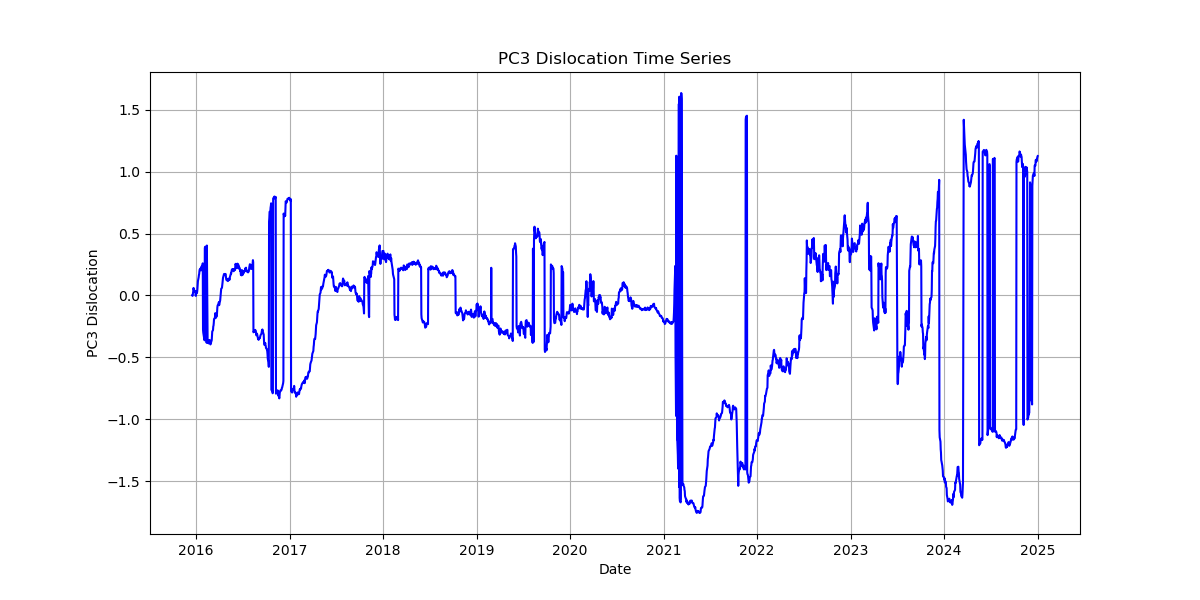
\includegraphics[width=0.8\textwidth]{visuals/pc3_dislocation_timeseries.png}
    \caption{PC3 Dislocation Time Series: Capturing curvature-driven distortions in mid-maturity yields over time.}
    \label{fig:pc3dislocation}
\end{figure}

\subsection{Application of the Fourier Transform}
To analyze the cyclical patterns inherent in the PC3 dislocation data, we apply the Discrete Fourier Transform (DFT). The DFT decomposes the time-domain signal into its constituent frequency components, allowing us to identify and quantify periodic behavior. The frequency spectrum generated from the Fourier Transform is displayed in Figure~\ref{fig:fullspectrum}.

\begin{figure}[H]
    \centering
    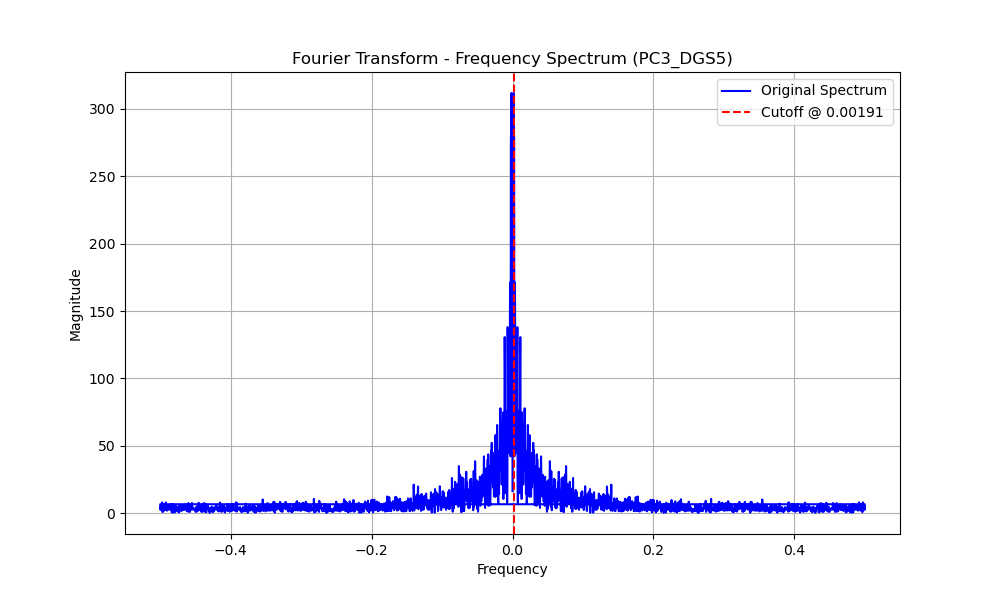
\includegraphics[width=0.8\textwidth]{visuals/fourier_full_spectrum.png}
    \caption{Fourier Transform - Full Frequency Spectrum of PC3 Dislocation.}
    \label{fig:fullspectrum}
\end{figure}

\subsubsection{Frequency Filtering}
While the full frequency spectrum provides a comprehensive view of all periodic components, our primary interest lies in the low-frequency region where long-term cyclical patterns reside. To isolate these components, we apply a frequency cutoff at 0.00191, determined empirically based on noise-to-signal analysis. Frequencies beyond this threshold are attenuated to remove short-term fluctuations, thereby enhancing the signal's stability. The filtered frequency spectrum, focusing on low frequencies, is shown in Figure~\ref{fig:zoomspectrum}.

The selection of the cutoff frequency is crucial for balancing noise reduction with trend preservation. To achieve this, we employ two primary methods:

\paragraph{1. Energy Threshold Method (85\% Variance Retention)}
The Energy Threshold Method selects a cutoff frequency by retaining the frequency components that account for at least 85\% of the total variance. This method ensures that the most influential frequencies are preserved while filtering out those with negligible contributions. To calculate this, we first determine the total energy of the signal as the sum of the squared magnitudes of the Fourier coefficients:
\[
E_{total} = \sum_{k=0}^{N-1} |X(k)|^2
\]

Next, we compute the cumulative energy up to each frequency \(f\) as follows:
\[
E(f) = \sum_{k=0}^{f} |X(k)|^2
\]

We then calculate the variance ratio at each frequency to identify the point where the cumulative energy first reaches 85\% of the total energy:
\[
\text{Variance Ratio} = \frac{E(f)}{E_{total}}
\]

\paragraph{2. Elbow Point Method (Diminishing Returns)}
The Elbow Point Method identifies the point at which the inclusion of additional frequency components leads to diminishing returns in variance retention. This is visually observed as a significant reduction in the slope of the cumulative variance curve, forming an "elbow" point. Selecting the frequency at this point ensures that only the most impactful components are retained without overfitting noise.

\paragraph{Conservative Approach: Minimum of Both Methods}
To balance between overfitting and underfitting, we take the conservative approach of selecting the minimum cutoff frequency derived from both methods. This choice prioritizes robustness by favoring the more restrictive cutoff, reducing the risk of retaining high-frequency noise while ensuring that critical long-term trends are preserved. This conservative strategy enhances the stability of the filtered signal and improves the reliability of trading signals derived from it.

\begin{figure}[H]
    \centering
    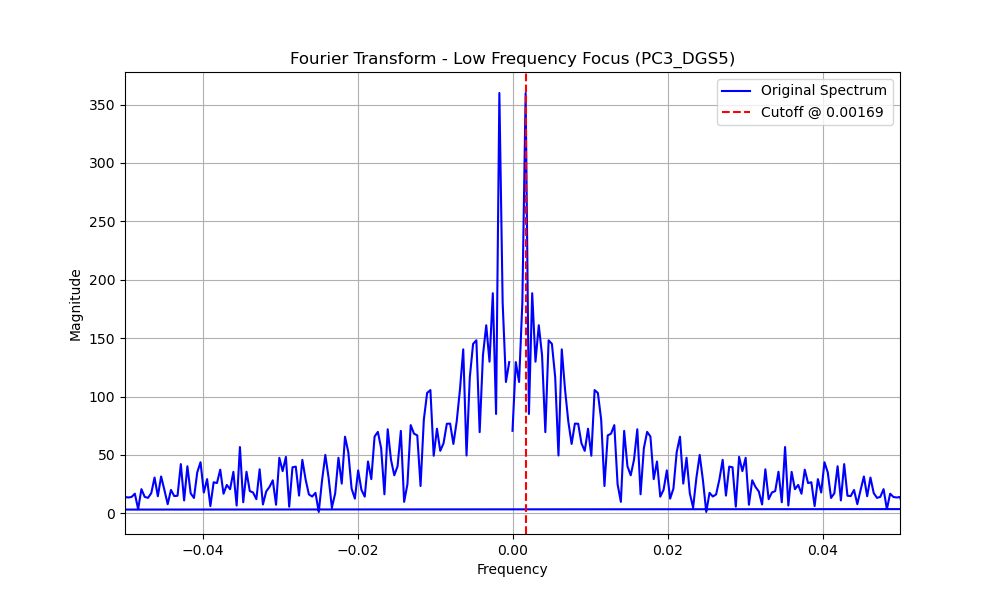
\includegraphics[width=0.8\textwidth]{visuals/fourier_zoomed_spectrum.png}
    \caption{Fourier Transform - Low Frequency Focus with Cutoff (0.00191).}
    \label{fig:zoomspectrum}
\end{figure}



\subsection{Signal Reconstruction}
After filtering out high-frequency components, the inverse Fourier Transform is applied to reconstruct the smoothed PC3 dislocation signal. This process yields a filtered time series that retains significant long-term cyclical patterns while minimizing noise. Figure~\ref{fig:filtered} shows the filtered signal compared to the original PC3 dislocation series.

\begin{figure}[H]
    \centering
    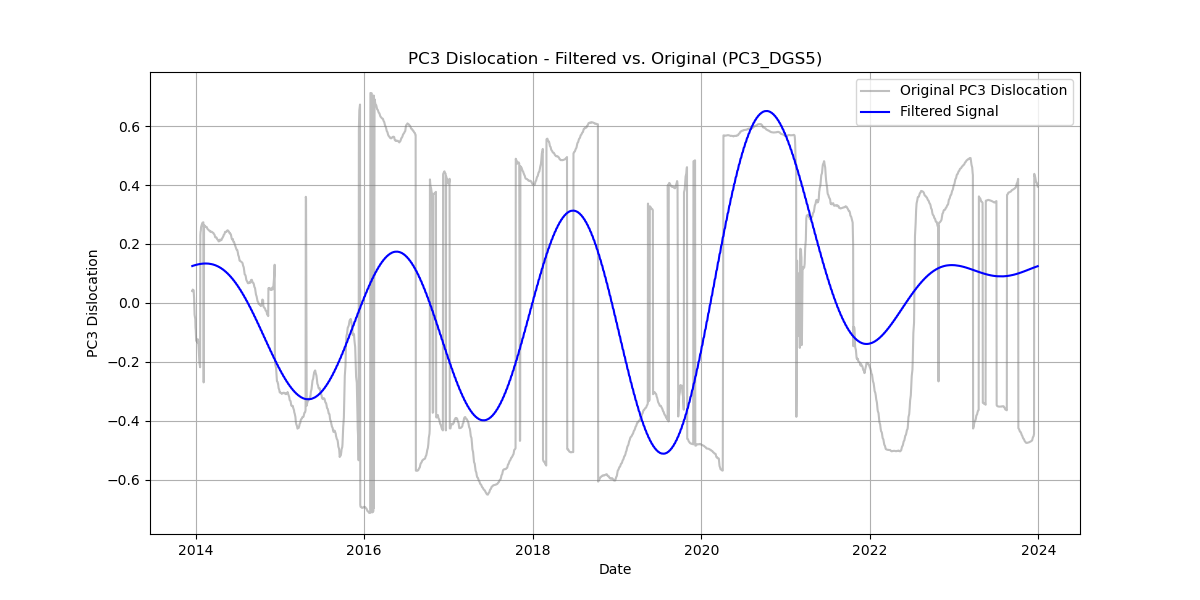
\includegraphics[width=0.8\textwidth]{visuals/fourier_filtered_signal.png}
    \caption{Filtered PC3 Dislocation Signal vs. Original Time Series.}
    \label{fig:filtered}
\end{figure}

\subsection{Interpretation and Significance}
The primary advantage of Fourier filtering is its ability to smooth PC3 dislocation signals by removing transient fluctuations that obscure true cyclical patterns. This refinement is essential for practical trading applications, as it reduces the likelihood of false signals triggered by noise. The resulting filtered signal highlights persistent mean-reverting behavior, which is fundamental for designing trading strategies that capitalize on curvature-driven arbitrage opportunities. By isolating long-term cycles and eliminating noise, Fourier Transform not only clarifies the nature of PC3 dislocations but also enhances the robustness of the arbitrage signals derived from them. This filtering approach complements our PCA methodology by ensuring that the final trading signals are based on significant, stable patterns rather than short-lived anomalies.

\section{Next Steps and Project Roadmap}

Having established a clean PC3 trading signal through Fourier filtering, and having demonstrated the mean-reverting behavior of PC3 dislocations across various market regimes, we are well-positioned to advance to the next stages of the project. These upcoming components will be integral to the final report and poster presentation, which will showcase the complete analysis and implementation of our arbitrage strategy. The next steps include:

\begin{enumerate}
    \item \textbf{Butterfly Hedges and Implementation:} 
    We will construct butterfly hedge trades specifically designed to isolate PC3 dislocations while neutralizing PC1 and PC2 exposure. This will involve precise calculation of hedge ratios to ensure that curvature-driven signals are exploited without being influenced by broader level or slope changes.

    \item \textbf{Backtesting Results:} 
    We will conduct thorough backtesting of the butterfly hedge strategy using historical data. This will allow us to evaluate the effectiveness and profitability of the approach over time, accounting for transaction costs and slippage. Performance metrics such as Sharpe ratio, maximum drawdown, and cumulative returns will be analyzed.

    \item \textbf{Forward Looking: Neural Networks, Reinforcement Learning, and Predictive Models:} 
    To further enhance trade timing and execution, we will explore the use of neural networks and reinforcement learning models. These predictive approaches will aim to improve signal accuracy and optimize trade entry and exit points, offering a forward-looking perspective on yield curve arbitrage.

\end{enumerate}

By systematically progressing through these next steps, we aim to demonstrate the full potential of the PC3-based arbitrage strategy and quantify its efficacy across various market conditions. The final presentation will synthesize these elements into a comprehensive analysis, illustrating both the theoretical foundations and practical implementation of our approach.







\end{document}